\chapter{Estado del arte}
Una vez introducido el proyecto y conocido sus objetivos es momento de realizar un análisis sobre el estado del arte para poder llevar a cabo una buena planificación posteriormente.

\section{Caso de estudio: Clínica Carmen Verdejo}
\begin{figure}[H]
    \centering{
\includegraphics[scale=0.15]{doc/imagenes/logo-carmen-verdejo.png}}
    \caption{Logo de la Clínica Carmen Verdejo}
    \label{fig:carmen-verdejo}
\end{figure}

Antes de analizar las herramientas actuales para la gestión online de citas es importante conocer la situación actual de la clínica Carmen Verdejo con el fin de establecer una perspectiva para dicho análisis.\bigskip

Para la obtención de información, además de consultar su página web se han formulado una serie de preguntas haciendo uso de la herramienta de Google Form \footnote{\url{https://docs.google.com/forms/d/1RtZ3cDxzFdChnDrg_rhbshSm4jA1VytI0ZoWE_Gb8mk/edit#response=ACYDBNjynGInGRGziJ00BEA2D9Pd-t9yG8e2FP8GdXHg3lbCqvj8Hxx9F-A0OLWGJ-g7Xos}}: \bigskip

\begin{itemize}
    \item Indique su grado de experiencia con Internet (en un intervalo de 0 a 5)
    \item Indique su grado de experiencia con dispositivos móviles (en un intervalo de 0 a 5)
    \item Indique su grado de experiencia con ordenadores (en un intervalo de 0 a 5)
    \item Indique su grado de experiencia con las redes sociales (en un intervalo de 0 a 5)
    \item Actualmente, ¿qué herramientas utiliza la clínica para gestionar las citas (registro, modificación, cancelación, notificación y consulta de citas) con los pacientes? Por ejemplo: Llamadas por teléfono, Google Calendar, Microsoft Excel, SMS, correo electrónico, WhatsApp, Telegram… 
    \item Indique el uso de cada una de las herramientas nombradas anteriormente. Por ejemplo: “Las llamadas por teléfono se utilizan para el registro, modificación, cancelación y consulta de citas; El registro, modificación y cancelación de citas se realizan por Google Calendar; La notificación de próximas citas a los pacientes se realiza por SMS”
    \item ¿Qué problemas o dificultades encontró al comenzar a utilizar las herramientas anteriores? Por ejemplo, “Google Calendar me pareció poco intuitivo para aprender”
    \item ¿Qué problemas o dificultades encuentra actualmente en el uso de las herramientas anteriores? Por ejemplo, “Hubo una confusión con la cita de un paciente”, “Es difícil cuadrar horarios con las disponibilidades de los pacientes”
    \item ¿Considera que cualquier persona (independientemente de su edad, experiencia con tecnologías o con una posible discapacidad como ceguera, parkinson, daltonismo…) sería capaz de gestionar las citas de la clínica correctamente con las herramientas actuales? ¿Por qué?
    \item ¿Considera que las herramientas utilizadas actualmente satisfacen las necesidades de la clínica para la gestión de citas? ¿Por qué?
    \item¿Qué posibles mejoras se podrían incorporar a las herramientas actuales? Por ejemplo, “ Se podrían enviar mensajes automáticamente a los pacientes vía Whatsaap para notificar su próxima cita”, “Se podrían guardar las disponibilidades de los pacientes para ser consultadas”
    \item¿Echa de menos otras funcionalidades en las herramientas actuales además de la gestión de citas? Si es así, ¿qué funcionalidades? Por ejemplo: “ Se podría añadir una funcionalidad para el registro de pagos de los pacientes”
\end{itemize}

La clínica Carmen Verdejo como se ha mencionado anteriormente en el capítulo \ref{intro} es una clínica de psicología ubicada en el Camino de los Abencerrajes 17 en Granada que cuenta con un equipo de entre x y x años y de pacientes entre x y x años PC. La labor diaria de la clínica es la de ofrecer los servicios de sus psicólogos para llevar a cabo diversos tipos de terapias adaptadas a sus pacientes y evidentemente para poder desempeñar correctamente esta labor se necesita de una agenda bien organizada.\bigskip

Carmen María Ramos Espejo, secretaria de la clínica, además de otras labores administrativas es la encargada de gestionar la agenda de la clínica atendiendo tanto las peticiones de los psicólogos, como las de los pacientes. Para ello, gran parte de su jornada laboral la invierte utilizando diversas herramientas para las siguientes tareas:

\begin{itemize}
    \item \textbf{Comunicación con los pacientes y el equipo para llevar a cabo registros, modificaciones, cancelaciones y recordatorios de citas}: WhatsApp, SMS y correo electrónico.
    \item \textbf{Gestión de citas del equipo de psicólogos}: Google Calendar.
\end{itemize}

La combinación de dichas herramientas, y por supuesto el contacto presencial más las llamadas telefónicas, permiten a Carmen María hacer una gestión de citas completa. Sin embargo, a pesar del uso de WhatsApp o Google Calendar esta metodología no se aleja mucho de la que podemos encontrar hace 20 años, ya que hemos cambiado el papel por un medio digital y añadido mensajes de texto. Por tanto, el flujo seguido a través de este procedimiento sigue siendo el mismo puesto que para realizar cualquier operación sobre una cita se sigue el siguiente esquema:

\begin{figure}[H]
    \centering{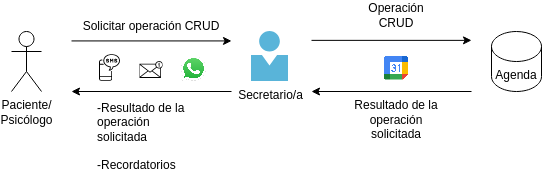
\includegraphics[scale=0.7]{doc/imagenes/flujo-tradicional.png}}
    \caption{Flujo tradicional adaptado a la Clínica Carmen Verdejo para la gestión de citas}
    \label{fig:flujo-tradicional}
\end{figure}

Observamos que un paciente o psicólogo para realizar cualquier gestión sobre sus citas siempre ha de pasar por un intermediario, quien se encarga de interactuar de forma directa con la agenda, en este caso Google Calendar. Es indiscutible que el hecho de que exista un intermediario ralentiza el proceso. Asimismo el canal de comunicación con el paciente puede conllevar a errores. \bigskip

A continuación se analizarán las herramientas utilizadas por la clínica para obtener una valoración de las mismas y determinar su utilidad en Carmen Verdejo.

\subsubsection*{Google Calendar}

\begin{figure}[H]
    \centering{
\includegraphics[scale=0.07]{doc/imagenes/google-calendar-logo.png}}
    \caption{Logo de Google Calendar}
    \label{fig:google-calendar}
\end{figure}

Google Calendar es un calendario online desarrollado por Google para uso personal o empresarial que permite la creación y compartición de eventos y reuniones o la planificación de tareas, así como notificar próximos eventos del calendario con tanta antelación como desee el usuario. \bigskip

Como ya se ha explicado, la clínica Carmen Verdejo utiliza Google Calendar a modo de agenda para gestionar las citas de los pacientes con el equipo de psicólogos. A este calendario sólo tiene acceso Carmen María quien es la única persona del equipo con el poder de crear, modificar, consultar o borrar citas, si alguno de los psicólogos desea realizar alguna de estas operaciones debe de solicitárselo a Carmen María. \bigskip

Tras conocer el uso de Google Calendar en la clínica, es momento de examinar la plataforma. En primer lugar hay que mencionar que un gran punto positivo es que es totalmente gratis, exceptuando su uso a través de SMS. Por supuesto también hay que destacar la experiencia de usuario ofrecida lo cual ya hizo Tanya Feddern-Beckan de la Escuela Miller de la Universidad de Miami en su artículo 'Google Calendar' \cite{FeddernBekcan2008}. Feddern resalta en lo referente a usabilidad, la alta personalización ofrecida: tamaño de fuente, idioma, formato de fecha y hora, zona horaria, colores... Adicionalmente la plataforma es totalmente responsiva adaptándose al tamaño de cualquier dispositivo y pudiendo funcionar en la mayoría de navegadores. Por otro lado, la personalización ya mencionada junto con el uso correcto de contrastes y grandes elementos visuales en los que hacer click la convierten en una aplicación bastante accesible para un gran abanico de tipos de usuario. \bigskip

Sin embargo, es tan profunda la personalización que puede llevarse a cabo en Google Calendar que un usuario con poca o media experiencia en el uso de este tipo de plataformas, desconoce las numerosas posibilidades que ofrece una herramienta tan potente. Un claro ejemplo de ello es el no uso de 'Calendarios Masters' en los que el usuario creador del calendario puede administrar los permisos que poseen los usuarios invitados al calendario. Esto permitiría que el resto del equipo no tuviera la necesidad de acudir a Carmen María para cualquier gestión sobre las citas. \bigskip

Queda claro con esta evaluación que Google Calendar es una muy buena herramienta para usar como agenda online para uso personal, pero no tanto para empresarial si los usuarios no están experimentados en el uso de este tipo de plataformas, por lo que en ese caso no es posible exprimir todo su potencial.

\subsubsection*{WhatsApp, correo electrónico y SMS}

WhatsApp, el correo electrónico y los SMS se tratan de servicios utilizados por la clínica Carmen Verdejo cuya combinación hace posible la comunicación a distancia con la mayoría de sus pacientes. Para los dos primeros se necesita acceso a Internet y ya se vio en el capítulo \ref{intro} que un 93.9\% de la población española entre 16 y 74 años usó Internet en el año 2021, de acuerdo a un estudio del INE. En cuanto a los SMS, un 99.5\% de la población en ese mismo estudio disponía de un teléfono móvil. Por lo cual el servicio de comunicación ofrecido por la clínica a sus pacientes es prácticamente accesible a todo el mundo. \bigskip

Sin embargo, a pesar de la extensión de su uso en España dichos medios de comunicación poseen desventajas, algunas de las cuales han sido destacadas por la clínica. Por ejemplo, el pago de los mensajes por SMS o la desconfianza generada por las alteraciones en la red que evoquen a un no correcto envío de los mensajes. Estas son algunas de las desventajas de las que un usuario medio es conocedor, no obstante un punto muy negativo que se ha de mencionar en este caso de estudio es el tratamiento de los datos por parte de WhatsApp y en el transporte de estos por parte de algunos proveedores de correo electrónico. \bigskip

Por una parte, WhatsApp es una aplicación de mensajería instantánea de la cual es propietaria actualmente Meta, una gran empresa estadounidense que ha sido causa de grandes polémicas en relación a la protección de datos. En lo que concierne a una clínica como Carmen Verdejo, que es un centro sanitario, el Servicio Nacional de Salud de Inglaterra no aconseja su uso en este tipo de centros \cite{Gould2016-ky}, ya que algo tan sensible como los datos de los pacientes han ser protegidos ante cualquier vulnerabilidad. \bigskip

Por otra parte, Carmen Verdejo utiliza Gmail y de acuerdo a la estadísticas de la Figura \ref{fig:cifrado-correo} obtenidas en los Informes de Transparencia de Google \footnote{\url{https://transparencyreport.google.com/safer-email/overview?hl=es}}, el envío constante de mensajes cifrados desde Gmail a otros proveedores no es constante tal y como se ve en la figura. Por tanto, si el paciente receptor de un mensaje utiliza otro proveedor distinto a Gmail, Gmail no se puede encargar del cifrado del correo en el envío.

\begin{figure}[H]
    \centering{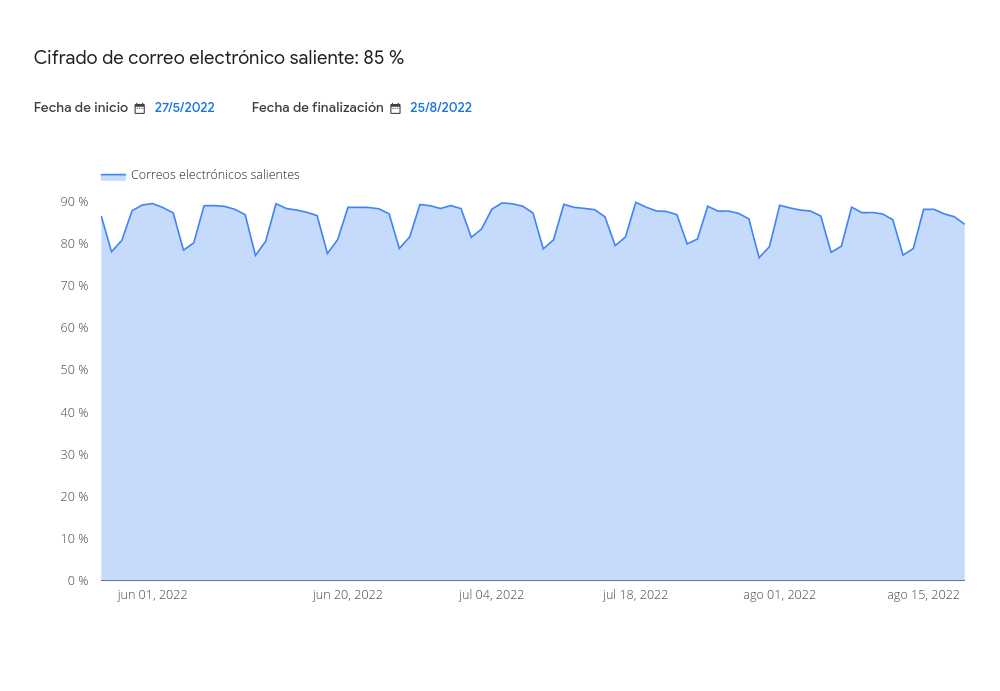
\includegraphics[scale=0.4]{doc/imagenes/cifrado-correo.png}}
    \caption{Cifrado de correo electrónico durante el envío de correo saliente en Google entre mayo y agosto de 2022}
    \label{fig:cifrado-correo}
\end{figure}

En definitiva, WhatsApp, el correo electrónico y los SMS son servicios muy completos, cómodos y útiles para la comunicación clínica-paciente, pero el peso de sus desventajas hace que se deba de considerar seriamente su sustitución por otros servicios de comunicación. 

\section{Soluciones para la gestión de citas online}
Después de haber conocido el día a día de la Clínica Carmen Verdejo en cuanto a la gestión de citas y las herramientas utilizadas para dicha labor, es momento de conocer otras opciones. Seguidamente, al igual que se ha hecho con las herramientas de Carmen Verdejo, se procede a realizar una evaluación de otros medios para la gestión de citas. Para ello se ha decidido analizar herramientas pensadas específicamente para la planificación de citas y herramientas genéricas de planificación cuyo fin no está especificado.

\subsection{Soluciones genéricas}

\subsubsection*{Notion}
\begin{figure}[H]
    \centering{
\includegraphics[scale=0.1]{doc/imagenes/notion-logo.png}}
    \caption{Logo de Notion}
    \label{fig:logo-notion}
\end{figure}

Notion \footnote{\url{https://www.notion.so}} es un software dirigido a la organización y planificación en cualquier marco de trabajo. A finales de 2021 acorde a la revista Forbes \footnote{\url{https://forbes.co/2021/10/11/emprendedores/notion-alcanza-una-valoracion-de-us10-000-millones-impulsada-por-el-trabajo-remoto-y-tiktok/}} ya contaba con más de 20 millones de usuarios, y es que esta plataforma conoce a la perfección qué necesita su público y cómo ofrecérselo. \bigskip

La plataforma hace uso de lo que ellos llaman \textit{Workspaces} \label{notion-workspaces} (espacios de trabajo) que son espacios colaborativos en los cuales un usuario o grupo de usuarios pueden gestionar su trabajo. Para lo cual se dispone de la creación de \textit{Páginas} que permiten al usuario crear una página en blanco o si se prefiere escoger entre una de las plantillas ofrecidas para crear una página como una lista de cosas por hacer, una agenda, un calendario, un tablero o incluso utilizarla como base de datos ya que permite la subida de archivos. Para mayor organización, se ofrece la posibilidad de almacenar páginas dentro de páginas, lo que equivaldría a disponer de carpetas. En adición a esto, con respecto a los espacios de trabajos Notion ofrece una jerarquía de usuarios diferenciando entre dos categorías:

\begin{itemize}
    \item \textbf{Usuarios internos al espacio de trabajo}: En este grupo de usuarios todos tienen acceso a todas las páginas del espacio de trabajo, así como editarlas y borrarlas, pero existe una subcategoría más que agrupa a los usuarios en dos grupos:
        \begin{itemize}
            \item \textbf{Administradores}: Aquellos que además de las funciones nombradas, pueden invitar o eliminar usuarios del espacio de trabajo, gestionar los pagos de éste y cambiar sus ajustes.
            \item \textbf{Miembros}: Sólo tienen permitido añadir, editar o eliminar páginas
        \end{itemize}
    
    \item \textbf{Usuarios externos al espacio de trabajo}: Notion denomina a este tipo de usuarios com o\textit{Guests} (huéspedes). Se tratan de usuarios que no pertencen al espacio de trabajo, pero que han sido invitados por un administrador a una o varias páginas. El administrador tiene la posibilidad de designar los privilegios de los que dispondrá el huesped sobre la página:.
        \begin{itemize}
            \item Compartir, editar y comentar
            \item Editar y comentar
            \item Comentar
            \item Sólo ver
        \end{itemize}
\end{itemize}

Adicionalmente cabe mencionar que cuenta con integraciones con Slack y Google Drive. \bigskip

Como se ha indicado es una herramienta destinada tanto para el uso individual como para el uso colaborativo de equipos y empresas. Sin embargo, la herramienta sólo es gratuita para uso individual con algunas limitaciones, si el usuario desea contar con más funcionalidades deberá de hacer la compra de uno de los planes que se muestran en la Figura \ref{fig:precios-notion}.

\begin{figure}[H]
    \centering{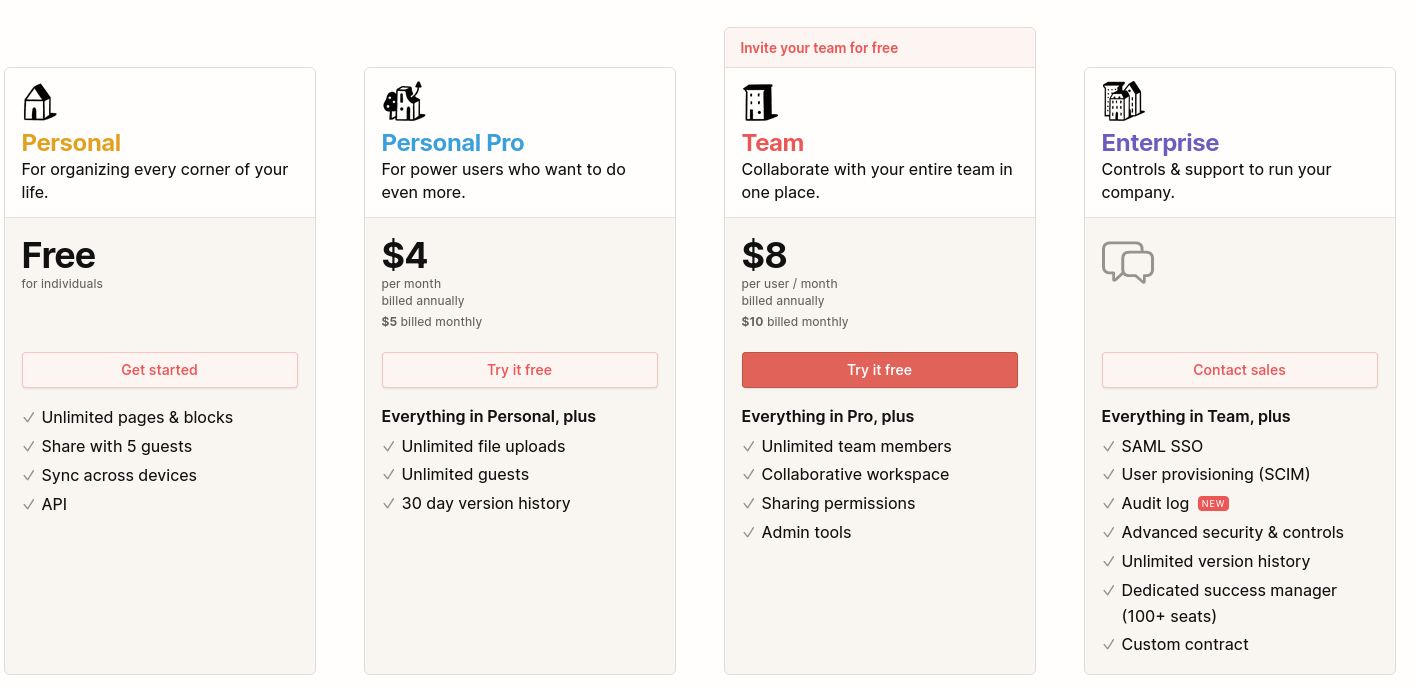
\includegraphics[scale=0.3]{doc/imagenes/precios-notion.png}}
    \caption{Planes de pago de Notion}
    \label{fig:precios-notion}
\end{figure}

En cuanto a lo que a Carmen Verdejo respecta con esta aplicación, la clínica podría hacer uso de la creación de páginas para que cada psicólogo dispusiera de una y dentro de dichas páginas se tuviera un calendario e información de las citas de todos sus pancientes. De esta forma agilizamos la comunicación psicólogo-secretaria de la Figura \ref{fig:flujo-tradicional}. Incluso a parte de la gestión de citas, la herramienta permitiría llevar un registro de pagos y documentación de los pacientes. Por otro lado, para la comunicación paciente-secretaria se tendría la posibilidad de añadir a los pacientes a su página correspondiente como huéspedes para gestionar sus citas, sólo se necesitaría que el paciente dispusiera de un correo electrónico para registrarse en Notion y conocimientos básicos en el uso de aplicaciones de este tipo. No obstante, aunque no dispusiera de esto último Notion tiene una guía \footnote{\url{https://www.notion.so/help/guides}} muy detallada sobre cómo usar la aplicación. \bigskip

Sin embargo, se ha indicado que para un trabajo colaborativo se debe de comprar uno de los dos planes de equipo, lo cual supone una importante cantidad de dinero al año teniendo en cuenta que el equipo está formado por x (PC) personas. Asimismo, otra desventaja de Notion es que sólo está disponible en inglés, francés, coreano y japonés, por lo que se da la posibilidad de que la plataforma no sea accesible para un determinado número de pacientes. \bigskip

En resumidas cuentas, Notion es una herramienta para la gestión de trabajo que ofrece infinitas posibilidades a sus usuarios para adaptar la herramienta a su ámbito de trabajo. Desde la clínica Carmen Verdejo ya se ha explicado cuál podría ser su papel en la gestión de citas, no obstante el alto precio a pagar y el idioma no compensa su uso. 

\subsubsection*{Asana}
\begin{figure}[H]
    \centering{
\includegraphics[scale=0.1]{doc/imagenes/asana-logo.png}}
    \caption{Logo de Asana}
    \label{fig:logo-asana}
\end{figure}

Asana \footnote{\url{https://app.asana.com}} es una plataforma desarrollada con objeto de ofrecer un servicio para gestionar el flujo de trabajo en equipos. A pesar de ello, es posible extender su uso a otros ámbitos como la gestión de citas online. \bigskip

La principal funcionalidad en el servicio brindado por Asana a sus usuarios es la creación de grupos de trabajos en los que los propios miembros del grupo pueden crear proyectos públicos para el resto del grupo o privados los cuales son sólo visibles a miembros del grupo invitados por el creador o por otros miembros que han sido invitados y tienen permisos de edición. Una vez que un proyecto ha sido creado, dentro del mismo los usuarios con permisos de edición pueden crear tareas organizadas por secciones cuya visibilidad puede ser controlada. En un proyecto los usuarios disponen de cuatro opciones para visualizar las tareas: en formato de calendario, como una lista, tablero o una línea temporal. Adicionalmente la plataforma ofrece reportes sobre el progreso de las tareas de un proyecto. \bigskip

Aparentemente Asana puede no parecer práctica para la planificación de citas, pero en realidad sí que se le puede sacar partido para ello, veamos a continuación cómo. La gestión de tareas con una fecha de entrega permite hacer una simulación en la que éstas se traten como citas y las secciones a las que pertenecen dichas ''tareas'' sean los pacientes en cuestión. Es decir, tendríamos tareas/citas asociadas a secciones/pacientes. Así mismo, se puede controlar la visibilidad de las citas para que cada psicólogo sólo tenga permisos de visualización y edición sobre las citas de sus pacientes y las pueda consultar a modo de agenda en el formato calendario de los proyectos. \bigskip

No obstante, Asana presenta algunos inconvenientes para su uso en la planificación de citas. Uno de estos inconvenientes es que a pesar del control de visibilidad que se puede aplicar sobre las tareas, las secciones no disponen de esta funcionalidad y los psicólogos tendrían visibles las secciones asociadas a pacientes que no son suyos. Añadido a esto, al comenzar a usar la herramienta su uso resulta muy poco intuitivo, en ningún momento se le explica al usuario los componentes de los que se forma la plataforma ni cómo usarlos. Por tanto, obligaría a éste a salir de la plataforma para buscar en su navegador tutoriales sobre su uso que son encontrados en la página oficial \footnote{\url{https://academy.asana.com/series/video-tutorials-tips}} , pero que desde dentro de la plataforma no son accesibles. \bigskip

Al igual que Notion, Asana dispone de tres planes a elegir para acceder a más y mejores funcionalidades. Entre ellas y la más importante para este análisis se encuentra la gestión de permisos. En la siguiente figura se muestran los precios junto con las funciones ofrecidas:

\begin{figure}[H]
    \centering{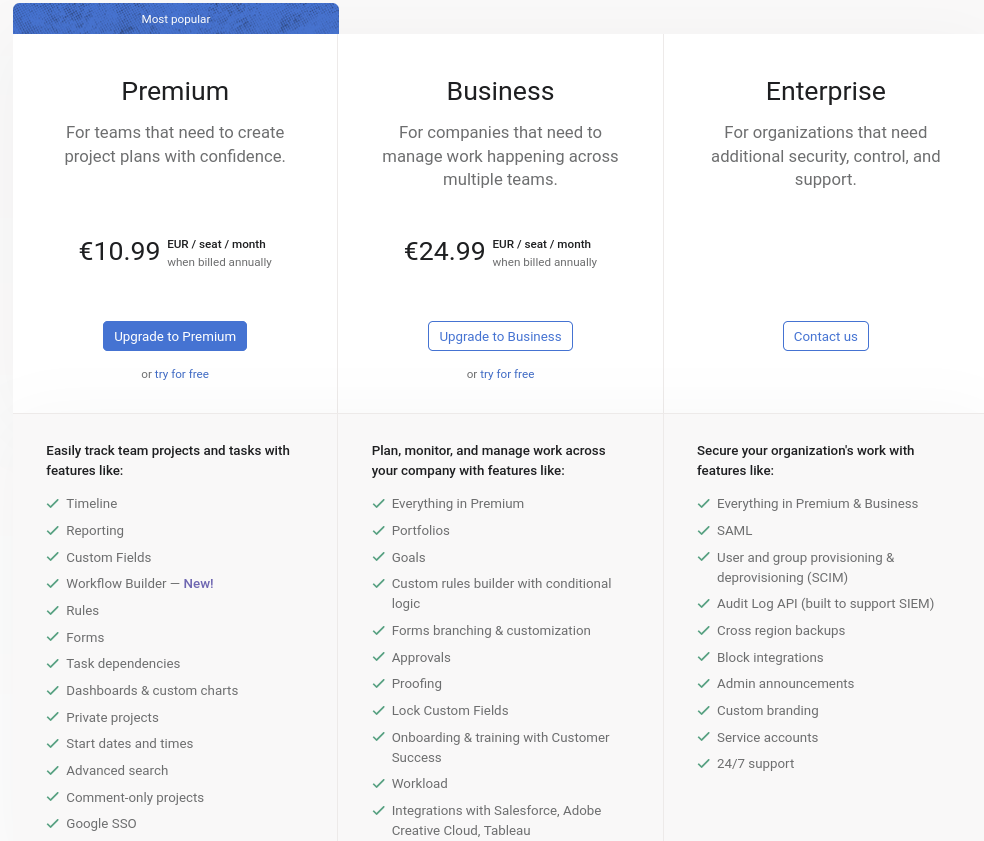
\includegraphics[scale=0.23]{doc/imagenes/asana-precios.png}}
    \caption{Planes de pago de Asana}
    \label{fig:asana-precios}
\end{figure}

Finalmente se ha de mencionar que la vía de comunicación psicólogo-secretario se vería mejorada, no obstante con Asana se hace muy difícil la adaptación para la comunicación paciente-secretario principalmente por la limitada gestión de permisos ofrecida en los packs. \bigskip

Con este análisis se concluye que Asana a pesar de ofrecer un servicio bastante aceptable para la gestión de citas resulta poco viable por su precio, limitaciones en la gestión de permisos y su imposibilidad para mejorar la comunicación paciente-secretario.


\subsubsection*{Trello}

\begin{figure}[H]
    \centering{
\includegraphics[scale=0.3]{doc/imagenes/trello-logo.png}}
    \caption{Logo de Trello}
    \label{fig:trello-logo}
\end{figure}

Trello \footnote{\url{https://trello.com}} es la plataforma por excelencia en la planificación digital de tareas para uso personal o corporativo.  A primera vista puede aparentar ser la herramienta que menos puede ofrecer en la gestión de citas entre todas las analizadas, pero está muy lejos de ello. Esta ''aparente sencillez'' resulta clave para que desde estudiantes hasta grandes multinacionales como Red Hat se decanten por utilizarla. \bigskip

La herramienta al igual que Notion presenta espacios de trabajo en los que el usuario dispone de la funcionalidad de creación y gestión de tableros. La visibilidad de los tableros puede ser restringida, para ello Trello distingue entre los siguientes tres niveles:

\begin{itemize}
    \item \textbf{Privado}: Sólo el creador y aquellos usuarios invitados pueden acceder y editar el tablero 
    \item \textbf{Espacio de trabajo}: El creador y los miembros del espacio de trabajo pueden acceder y editar el tablero
    \item \textbf{Público}: Todo el mundo tiene acceso al tablero, pero sólo los miembros del espacio de trabajo pueden editarlo.
\end{itemize}

Dentro de los tableros los usuarios crean \textbf{tarjetas} que son organizadas en \textbf{listas}. A cada tarjeta se le puede asignar un usuario con acceso al tablero, una fecha, archivos o etiquetas, además de poder personalizar su aspecto. No sólo eso, sino que también se puede decidir si recibir notificaciones cuando una tarjeta cambia su estado. También resulta relevante mencionar que Trello ofrece integraciones gratuitas con otras plataformas entre las que se encuentra Google Calendar. \bigskip

Por una lado, como se ha indicado Trello presenta integraciones entre las que se encuentra Google Calendar, lo cual resulta muy interesante para la clínica Carmen Verdejo que ya utiliza Google Calendar. Por otro lado, los psicólogos dispondrían de su propia ''agenda'' en forma de tablero con las citas de sus pacientes en forma de tarjetas gestionables tanto por la secretaria como por el psicólogo. Por tanto, la combinación del uso de Google Calendar y Trello abriría la posibilidad de que no sólo los psicólogos consultaran sus citas tanto por Trello como por Google Calendar, sino que también los propios pacientes pudieran hacerlo con la gestión de permisos ofrecida por Google Calendar y sus ''Calendarios Master''. \bigskip

Al igual que las otras dos soluciones, Trello cuenta los siguientes planes de pago en la Figura \ref{fig:trello-precios} para una mejora de las funcionalidades ofrecidas. 

\begin{figure}[H]
    \centering{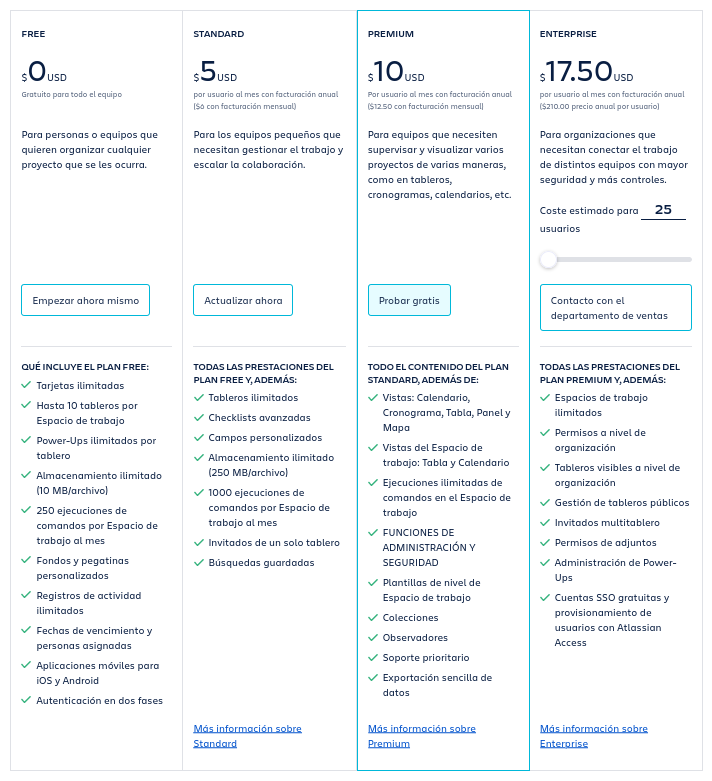
\includegraphics[scale=0.4]{doc/imagenes/precios-trello.png}}
    \caption{Planes de pago en Trello}
    \label{fig:trello-precios}
\end{figure}

Visualizando estos planes es evidente que para planificación de citas, el plan gratuito no es suficiente y en función del número de miembros del equipo de la clínica se tendría que optar por un plan de pago u otro. Seguidamente se explica por qué es conveniente en este caso decidirse por uno de los planes. \bigskip

Para empezar, por el limitado número de tableros ofrecidos en el plan gratuito, diez, ya que lo óptimo para su uso en la gestión de citas sería la creación de un tablero por psicólogo en el que cada tarjeta se asociara a una cita con un paciente. En adición a los planes de pago, si se quieren visualizar las tarjetas con otros formatos, como un calendario, se ha de contratar el plan Premium. Además, a pesar de las mejoras en la jerarquía de permisos, la jerarquía sólo se aplica a nivel de tablero, por lo que los pacientes no tendrían la posibilidad de hacer uso de Trello debido a que en dicha jerarquía aquel usuario invitado a un tablero independientemente de si puede editar o no, se le permite ver todas las tarjetas. Por tanto, un paciente vería las citas de otros pacientes y esto no se debe de permitir. Por tanto, para construir una agenda online con Trello mínimo se deberían de pagar aproximadamente diez euros mensuales por usuario. \bigskip

Definitivamente Trello resulta muy atractiva como solución con la integración gratuita de Google Calendar. No obstante, a pesar de su sencillo uso volveríamos a enfrentarnos con los mismos obstáculos presentados por Google Calendar para usuarios poco experimentados en el uso de estas plataformas y añadido a esto el gasto por un plan de pago para poder llevar a cabo la gestión de citas correctamente. Es por ello que su uso para este cometido no sería viable.


\subsection{Soluciones específicas}

\subsubsection*{ProDocfav}

\begin{figure}[H]
    \centering{
\includegraphics[scale=0.1]{doc/imagenes/logo-docfav.jpg}}
    \caption{Logo de ProDocfav}
    \label{fig:docfav-logo}
\end{figure}

ProDocfav \footnote{\url{https://pro.docfav.com/}} se ha elegido como la primera solución específica a analizar debido a que la clínica Carmen Verdejo se encuentra actualmente valorando su incorporación en su gestión de citas. \bigskip

Se trata de un software para clínicas perteneciente a la empresa vizcaína Docfav. Como la empresa indica en su página web oficial, tiene el propósito de gestionar el ciclo completo del paciente, es decir, no sólo las citas, sino también historial clínico, facturación e incluso la realización de consultas por videollamada. Por lo que Docfav promete ofrecer un servicio 360º en la gestión de pacientes. \bigskip

Para este análisis se va a utilizar su versión Demo gratuita que a pesar de tener una funcionalidad limitada, se puede recopilar más información acerca de su uso gracias a su manual de usuario \footnote{\url{ https://docfav.gitbook.io/docfav/}} que es público para todo el mundo . \bigskip

La plataforma tal y como se presenta resulta muy intuitiva a primera vista, pues en su vista principal el flujo seguido por sus usuarios (tanto profesionales, como pacientes) gira alrededor de la funcionalidad principal, la gestión de citas. Acompañada de una interfaz bastante agradable, el foco se pone en un calendario (Figura \ref{fig:docfav-calendario}) en el que se puede llevar a cabo la planificación de citas de los pacientes, pudiendo filtrar entre las agendas de los miembros de la clínica, los pacientes o los distintos servicios ofrecidos. Presenta un menú lateral que nos ofrece navegar a las secciones de gestión de clientes, facturación, estadísticas y ajustes, así como a la página externa correspondiente al manual del usuario. Cabe también mencionar que el software cuenta con integraciones con los calendarios de Google, Outlook, Apple... \bigskip

\begin{figure}[H]
    \centering{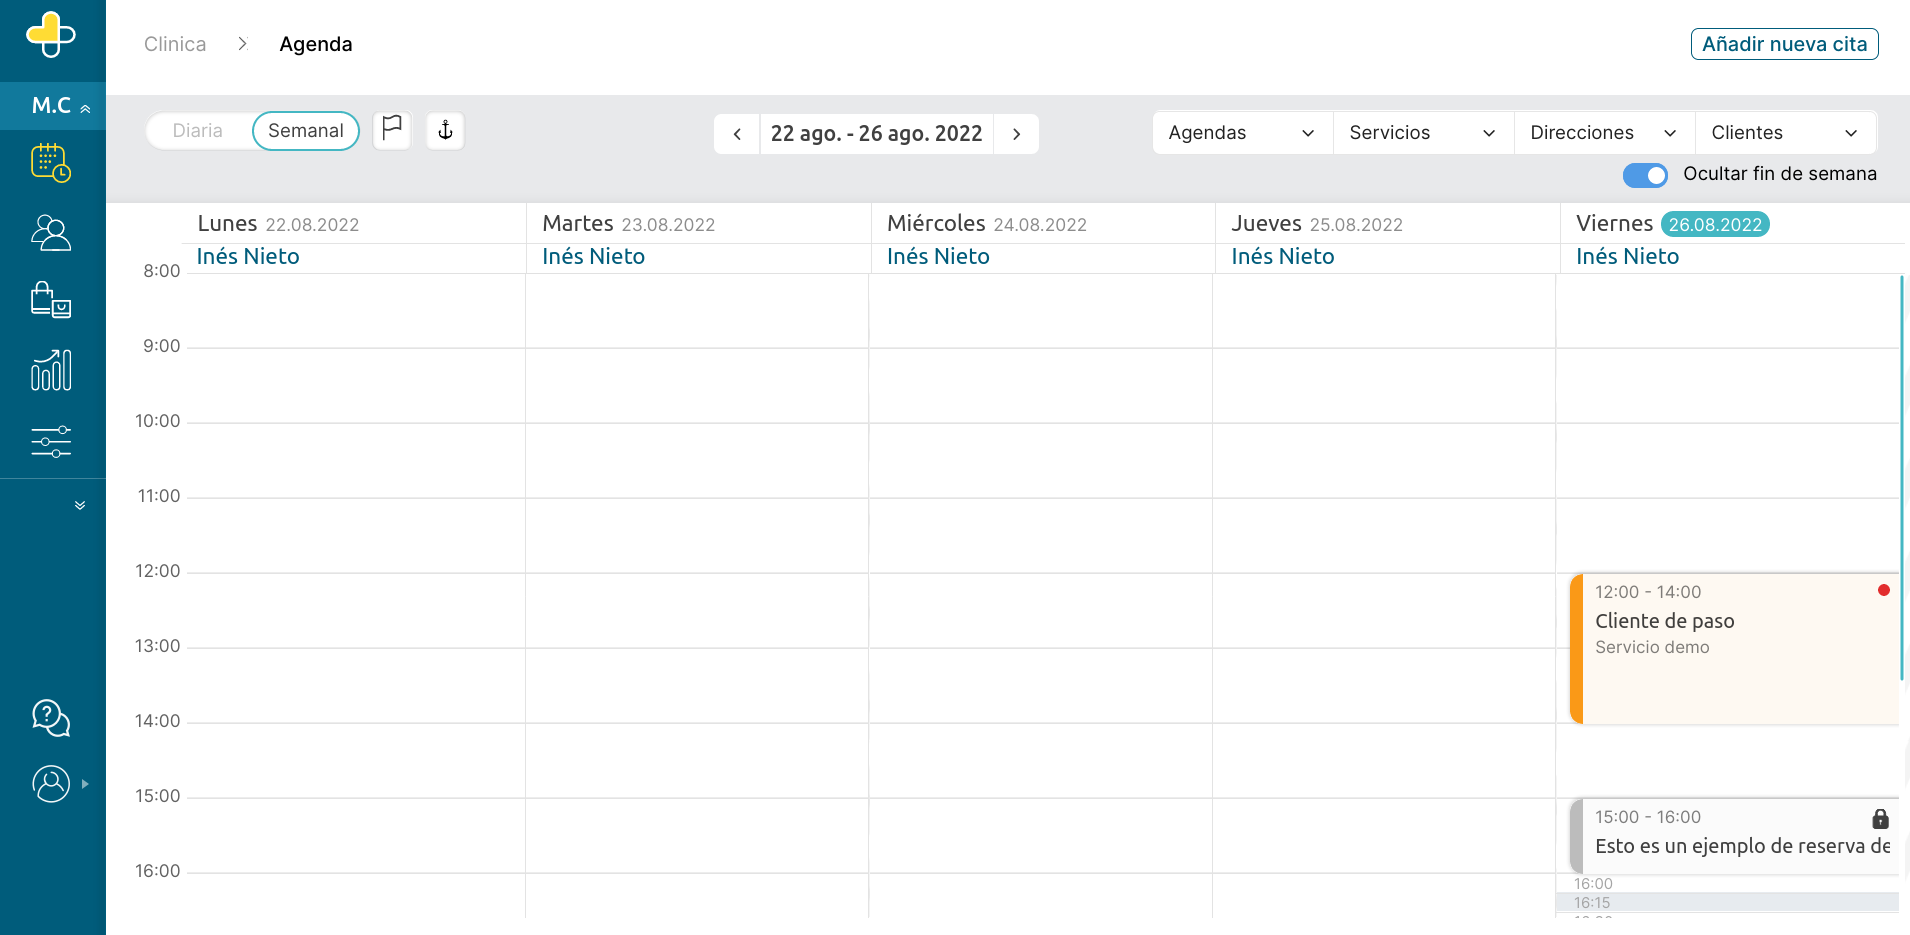
\includegraphics[scale=0.2]{doc/imagenes/docfav-calendario.png}}
    \caption{Sección principal de ProDocfav}
    \label{fig:docfav-calendario}
\end{figure}

Tras hacer una navegación por la plataforma y probar sus distintas funcionalidades, exceptuando la gestión del calendario, el resto de vistas se encuentran saturadas y no se aprecia ningún tipo de jerarquía visual, por ejemplo esto se puede comprobar en la vista de facturación, Figura \ref{fig:facturacion-docfav}:

\begin{figure}[H]
    \centering{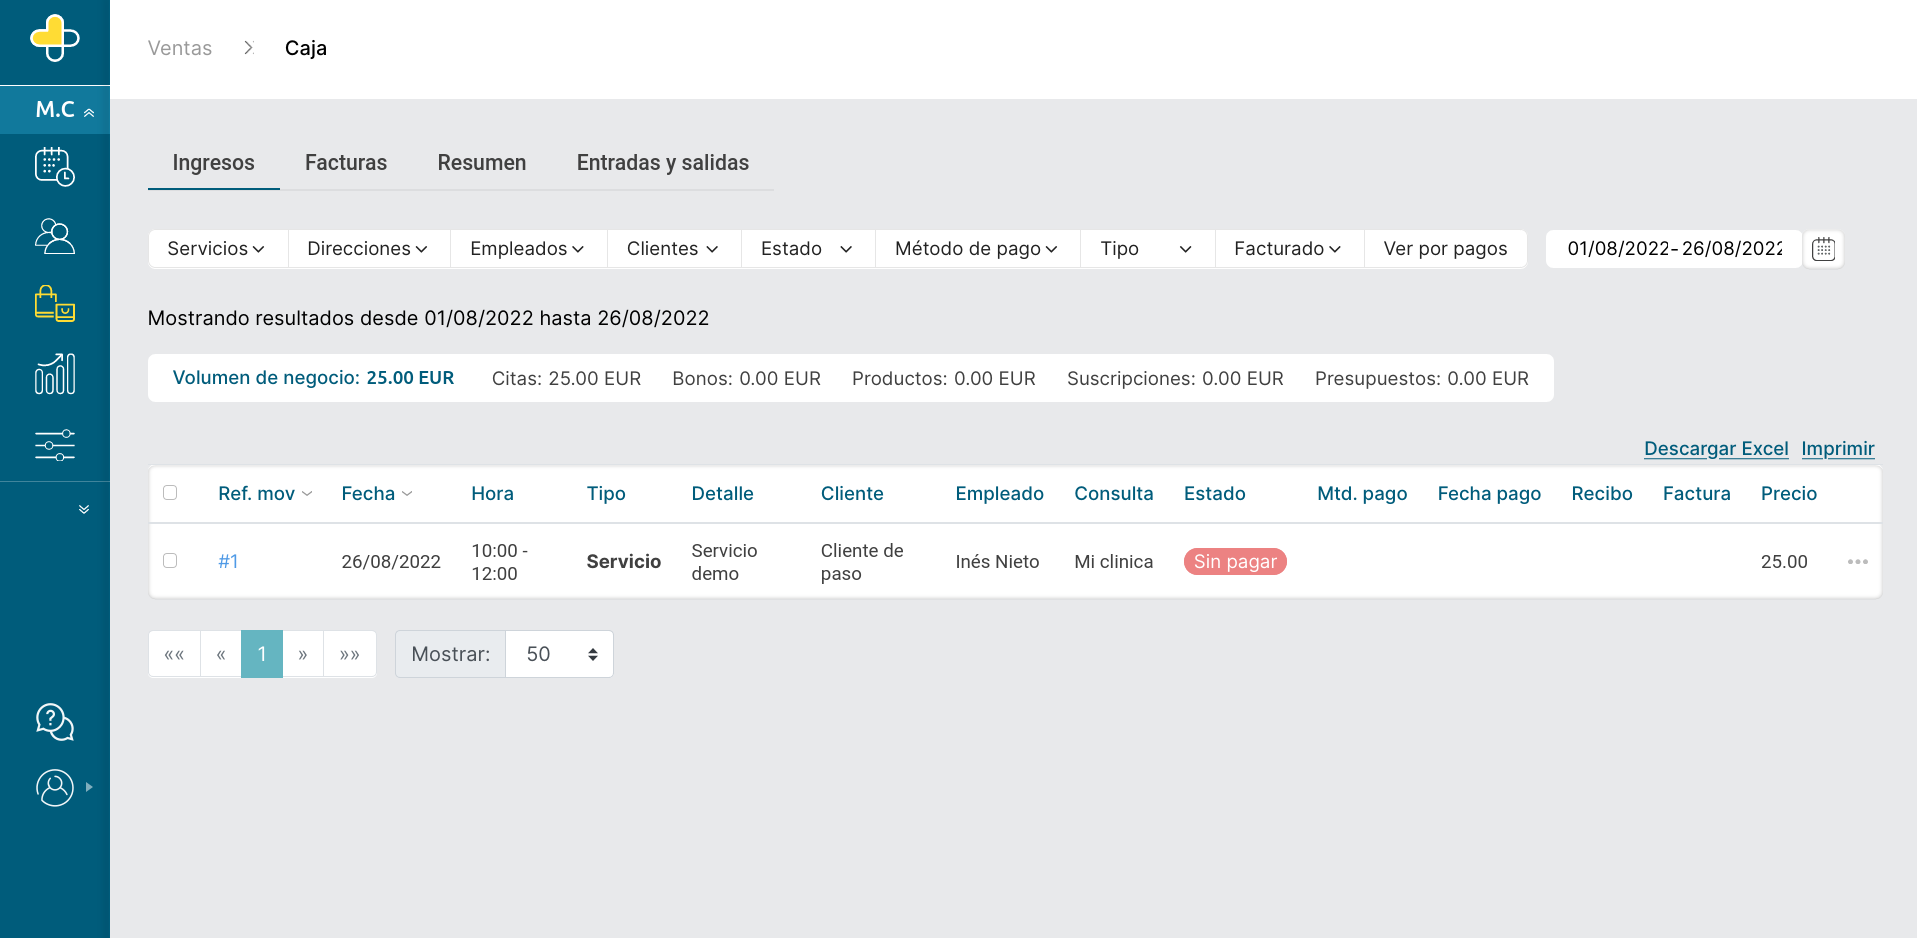
\includegraphics[scale=0.2]{doc/imagenes/facturacion-docfav.png}}
    \caption{Sección de facturación de ProDocfav}
    \label{fig:facturacion-docfav}
\end{figure}

De igual forma ocurre en la vista de los ajustes donde no se organizan las distintas acciones a realizar (Figura \ref{fig:ajustes-docfav}) y tan sólo se muestra un listado. Esto provoca a que el menú presentado resulte realmente incómodo de leer, pues de acuerdo a los principios de experiencia de usuario \cite{Scott2009-dh} para el ojo humano es mucho más fácil leer en vertical que en horizontal. Adicionalmente, debería de ser suficiente con leer el título de una opción del menú y no sobrecargar la vista con demasiado texto explicativo, como ocurre en este caso. 

\begin{figure}[H]
    \centering{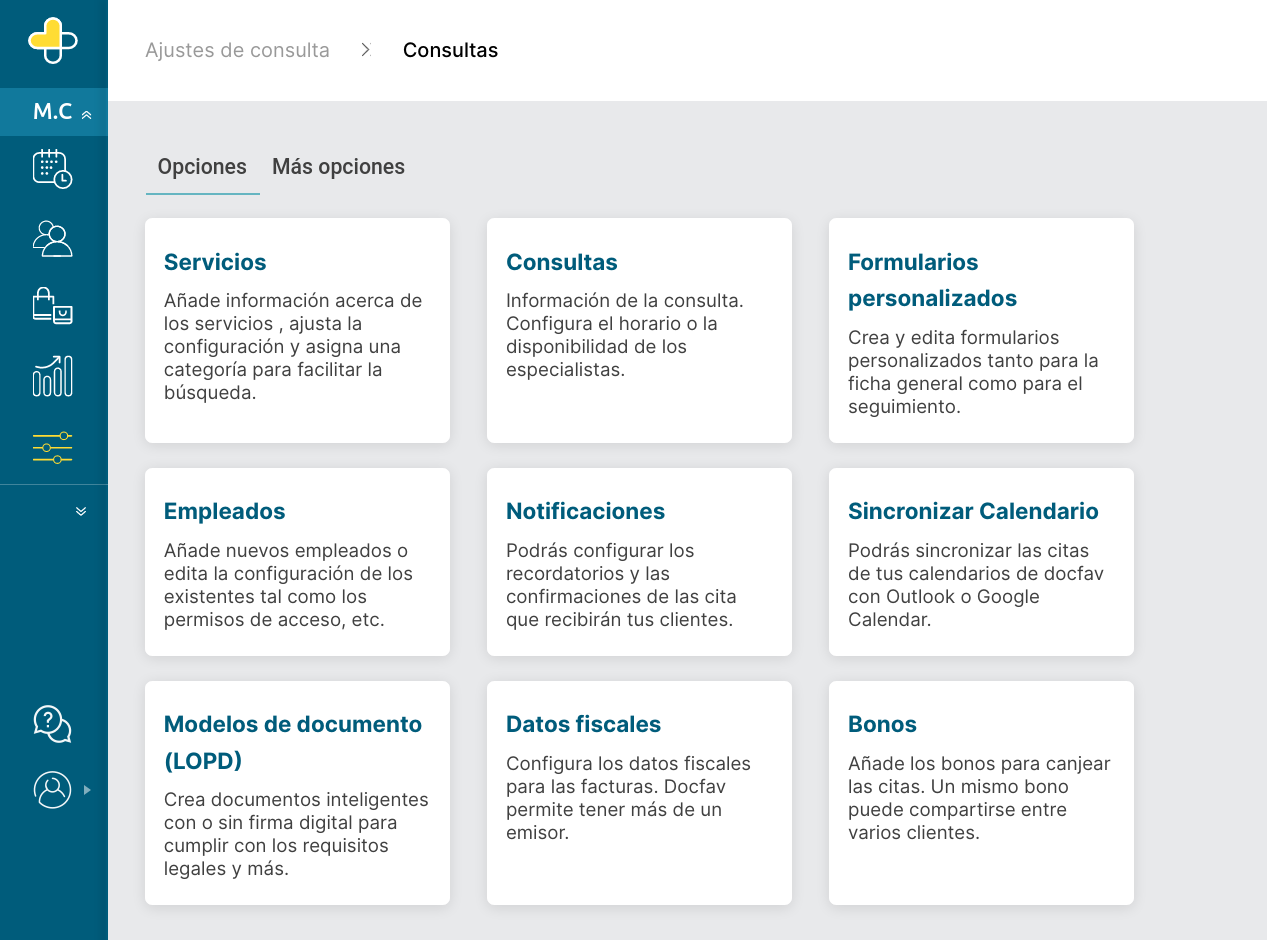
\includegraphics[scale=0.2]{doc/imagenes/docfav-ajustes.png}}
    \caption{Sección de ajustes de ProDocfav}
    \label{fig:ajustes-docfav}
\end{figure}

No obstante, estos defectos en el diseño de la interfaz que evocan a posibles confusiones en el uso de la plataforma se ven ligeramente compensados por la ayuda aportada por DocFav en su detallado manual del usuario. \bigskip

En cuanto al plan de precios, ProDocfav ofrece un sólo plan de pago de precio variante en función del número de trabajadores que utilicen el software. Por ejemplo, para diez trabajadores el precio a pagar de forma anual es de 62.42€ y de forma mensual de 74.90€. Desde luego un precio bastante alto en comparación a los planes de pago de las herramientas no específicas. \bigskip

En resumidas cuentas, ProDocfav a nivel de funcionalidad cubre con todas las necesidades que una clínica requiere para la gestión de sus citas y documentación. Sin embargo, parte de ese potencial se disipa si la experiencia de usuario acaba no siendo la mejor posible y más aún si no cumple con las expectativas de lo que se espera de un software de calidad de más de 60€ para diez usuarios. 

\subsubsection*{DriCloud}

\begin{figure}[H]
    \centering{
\includegraphics[scale=0.4]{doc/imagenes/dricloud-logo.png}}
    \caption{Logo de DriCloud}
    \label{fig:dricloud-logo}
\end{figure}

DriCloud \footnote{\url{https://dricloud.com/}} se define a sí mismo como  el mejor programa médico en la nube líder en 18 países. Sin duda alguna se trata de una contudente presentación que en pocas palabras suscita a cualquier usuario a tener grandes expectivas sobre este software. Es más, estas expectativas crecen aún más al conocer que instituciones de renombre como el Instituto Madrileño de Traumatología o el Instituto Andaluz de Neurología Pediátrica apuestan por su uso. \bigskip

Al igual que en el anterior caso, para el análisis de DriCloud se hará uso de la Demo proporcionada por la plataforma. No obstante, en este caso la demo está formada por una serie de vídeos explicativos sobre su uso. \bigskip

DriCloud ofrece gestión de citas de pacientes, de documentación (presupuestos, facturas, historiales clínicos...), guardado de firma digital, gestión de vacaciones de los trabajadores, creación de formularios de historia clínica,etc. Es decir, no sólo ofrece funcionalidades para la gestión de los pacientes, sino también funcionalidades para la gestión interna de la clínica. \bigskip

Dentro de la plataforma se distinguen una serie de roles para controlar las vistas a las que tiene permitido acceder un usuario. De acuerdo al video explicativo estos roles son los siguientes:

\begin{itemize}
    \item \textbf{Administrador del software}
    \item \textbf{Director}
    \item \textbf{Profesional}
    \item \textbf{Técnico} 
    \item \textbf{Secretaria}
    \item \textbf{Enfermera}
    \item \textbf{Contable}
\end{itemize}

Es importante mencionar que no existe una jerarquía explícitamente en la plataforma. Cada rol tiene asignadas unas vistas a las que puede acceder totalmente diferentes a las que tienen el resto de roles, por lo que si por ejemplo se desea crear un superusuario el usuario debe de tener todos los roles asignados. \bigskip

Centrándonos en el propósito que concierne a este proyecto, la gestión de citas online, DriCloud ofrece a los profesionales una \textit{Agenda}: 

\begin{figure}[H]
    \centering{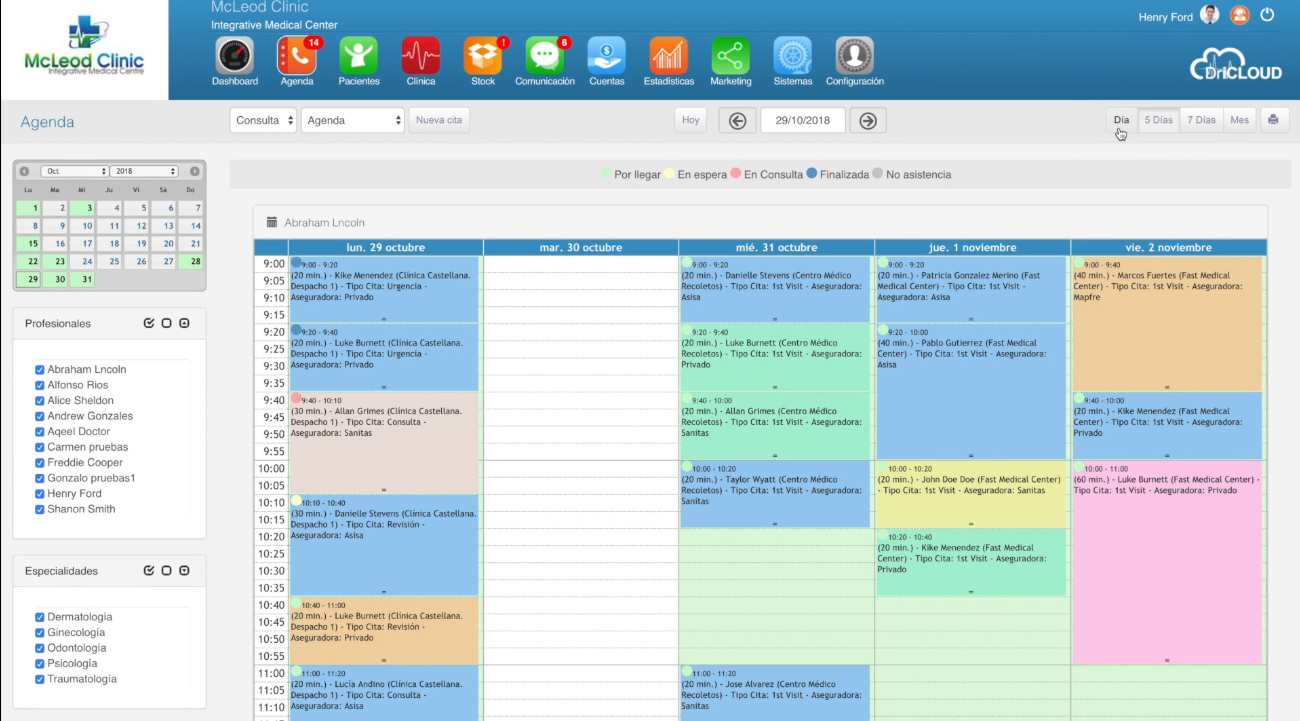
\includegraphics[scale=0.3]{doc/imagenes/dricloud-principal.png}}
    \caption{Vista principal de DriCloud para trabajadores}
    \label{fig:dricloud-principal}
\end{figure}

En esta agenda son destacables las siguientes características:

\begin{itemize}
    \item Las citas tienen asociado un estado (''Por llegar'',''En consulta'',''Finalizada'' y ''No asistencia'').
    \item Se da la opción de visualizar citas del día actual, los próximos cinco días, los próximos siete días o del resto del mes.
    \item Las citas pueden ser filtradas por profesional y/o especialidad.
    \item Dispone de tres modos de visualización:
    \begin{itemize}
        \item El modo \textbf{''Consulta''} que es el de la Figura \ref{fig:dricloud-principal}.
        \item El modo \textbf{''Planning''} en el que las citas se disponen como una línea temporal.
        \item El modo \textbf{''Dietario''} en el cual la información de las citas es mostrada en una tabla.
    \end{itemize}
\end{itemize}

En cuanto a los pacientes, DriCloud ofrece a sus clientes un código HTML para insertar en sus páginas un botón que permita realizar citas online. Este botón abre un formulario implementado por su equipo de desarrollo que el paciente deberá de rellenar para pedir una cita. Una vez el formulario haya sido enviado se le notifica la información de la cita al paciente vía SMS e email y dicha cita se crea en la agenda asociada al profesional que le atenderá. \bigskip

El servicio ofrecido a nivel funcional por DriCloud resulta realmente profundo, no sólo se puede hacer una gestión de citas y documentación de los pacientes, sino también del personal hasta el punto de hacer gestiones de recursos humanos como son la planificación de vacaciones. \bigskip

En lo que refiere a cuánto hay que pagar para acceder a estos servicios, se tienen varios planes de pago (Figura \ref{fig:dricloud-precios}). Si tomamos de referencia el plan de pago de ProDocfav, los precios son justificables ya que la plataforma ofrece más servicios. \bigskip

\begin{figure}[H]
    \centering{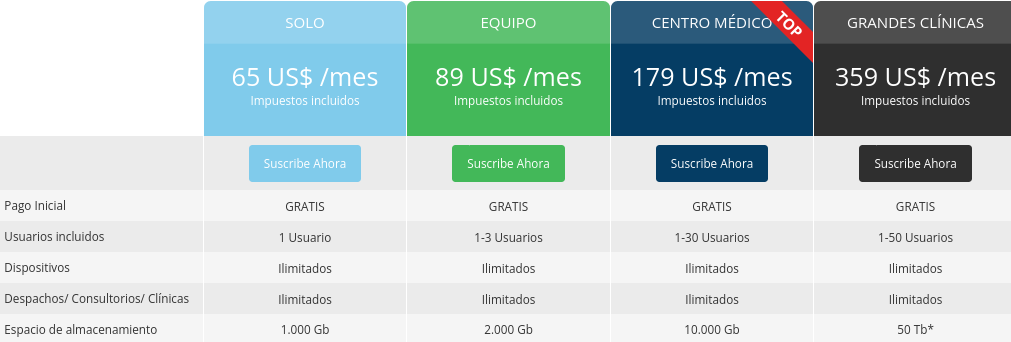
\includegraphics[scale=0.3]{doc/imagenes/dricloud-precios.png}}
    \caption{Planes de pago de DriCloud}
    \label{fig:dricloud-precios}
\end{figure}

Es claro que como usuario primerizo en la plataforma sin la ayuda ofrecida en los videos explicativos, resulta muy complicado entender su funcionamiento debido a las tantas funcionalidades proporcionadas. Se ha hecho durante los análisis anteriores bastante hincapié en el diseño de las interfaces, su usabilidad y accesibilidad ya que por muy buena y completa sea la funcionalidad ofrecida por una plataforma de nada sirve si no se le proporciona de forma correcta al usuario dicha funcionalidad. En esta herramienta encontramos al igual que en ProDocfav una importante saturación de la vista con texto innecesario (como el del menú de iconos o la leyenda de colores), iconos grandes y complejos, la no existencia de una jerarquía visual y el no uso de una paleta de colores. También hay que mencionar el uso del femenino en los roles \textit{Secretaria} y \textit{Enfermera} lo cual denota cierto sexismo. Se trata por tanto de una interfaz muy mejorable. \bigskip

El servicio de 24 horas proporcionado a los pacientes para solicitar una cita y el posterior envío de un SMS e email es un punto muy positivo, pero es incompleto ya que para modificar una cita, o incluso su consulta si se eliminase ese SMS o email, el paciente se debería de poner en contacto con la clínica.\bigskip

Para concluir, es evidente que una clínica como Carmen Verdejo conformada por PC x profesionales no le sacaría partido a esta herramienta. El plan de pago por el que se tendría que optar sería el de 179 euros mensuales para puedan acceder entre 1-30 usuarios y esto obliga a contratar un espacio de almacenamiento de 10 000Gb. Se trata pagar por un servicio que cubre mucho más allá de las necesidades de la clínica para finalmente seguramente no utilizar ni casi la mitad de todo lo ofrecido en dicho servicio. Para empresas y clínicas más grandes con varios establecimientos sí valdría la pena, pero en el caso de estudio de este proyecto definitivamente no.

\subsubsection*{Archivex}

\begin{figure}[H]
    \centering{
\includegraphics[scale=0.7]{doc/imagenes/archivex-logo.jpg
    }}
    \caption{Logo de Archivex}
    \label{fig:archivex-logo}
\end{figure}

 Archivex \footnote{\url{https://archivexclinical.com/}} es un software de gestión de clínicas desarrollado por Xoborg Technologies S.L en Salamanca. En su página oficial prometen que con el uso de Archivex la gestión de las clínicas de sus clientes se convertirá en un proceso sencillo en el que se ahorrará tiempo y dinero. Para evaluar la veracidad de estas palabras se hará uso de la demo ofrecida de siete días, así como de los vídeos explicativos disponibles en su canal de Youtube \footnote{\url{https://www.youtube.com/channel/UCGYoa8th_3iIZk1Zk9OGJTA}}. \bigskip

Archivex puede utilizarse en ordenadores con sistema operativo Windows o macOs, tablets y móviles Android o iOS. La plataforma al igual que el resto de soluciones anteriores, pone el foco de su vista principal en la agenda de sus profesionales, pero con algunas diferencias. En su vista principal llamada ''Hoy'' (Figura \ref{fig:archivex-principal} ) se presenta al usuario el personal de la clínica junto con la hora y paciente de su próxima cita si la hubiera. Si se hace click sobre uno de los profesionales, el usuario navegaría a la agenda semanal del profesional seleccionado (Figura \ref{fig:archivex-agenda-profesional} ). 

\begin{figure}[H]
    \centering{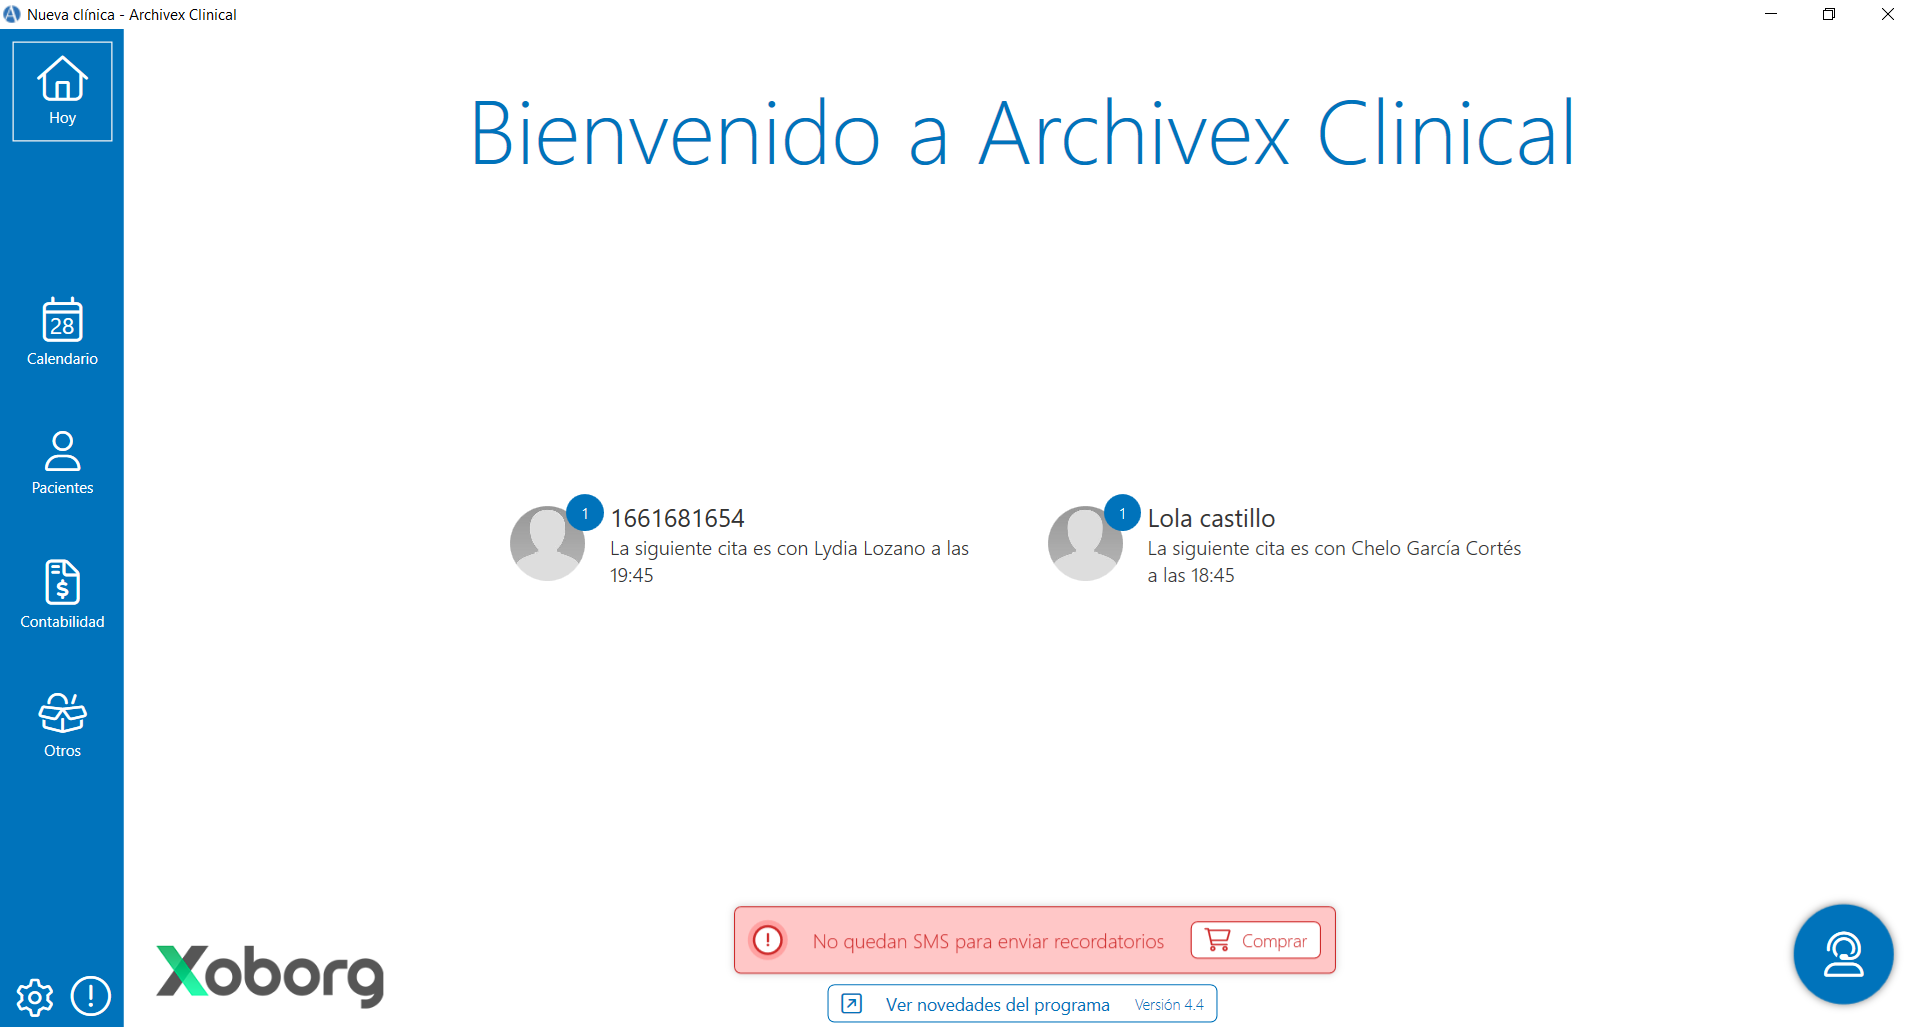
\includegraphics[scale=0.3]{doc/imagenes/archivex-principal.png
    }}
    \caption{Vista principal de Archivex}
    \label{fig:archivex-principal}
\end{figure}

\begin{figure}[H]
    \centering{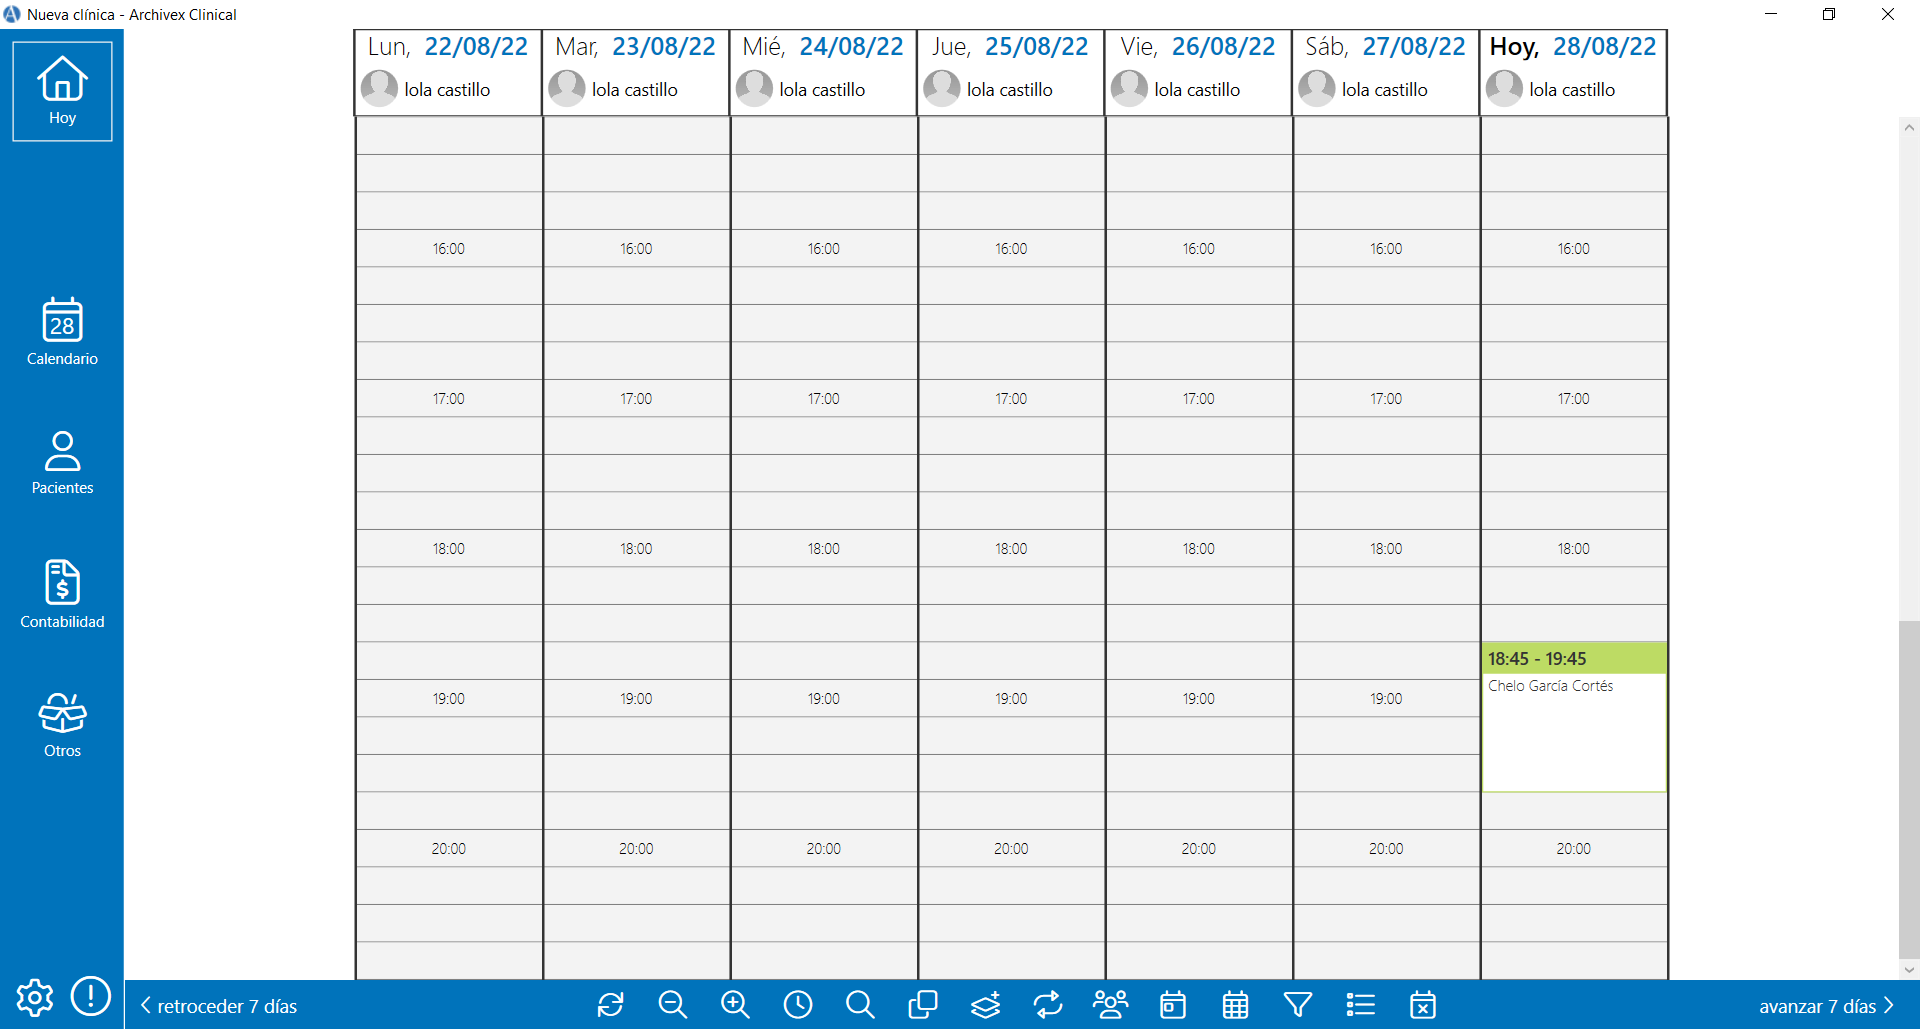
\includegraphics[scale=0.3]{doc/imagenes/archivex-agenda-profesional.png
    }}
    \caption{Vista semanal de la agenda de un profesional Archivex}
    \label{fig:archivex-agenda-profesional}
\end{figure}

En cuanto a la vista del ''Calendario'' (Figura \ref{fig:archivex-calendario}), nuevamente el usuario se toparía con la elección de escoger a uno de los profesionales para navegar a la vista de la Figura \ref{fig:archivex-agenda-profesional}. Además, tiene también la posibilidad de visualizar las citas por día de todos los profesionales (Figura \ref{fig:archivex-agenda-todos}  )

\begin{figure}[H]
    \centering{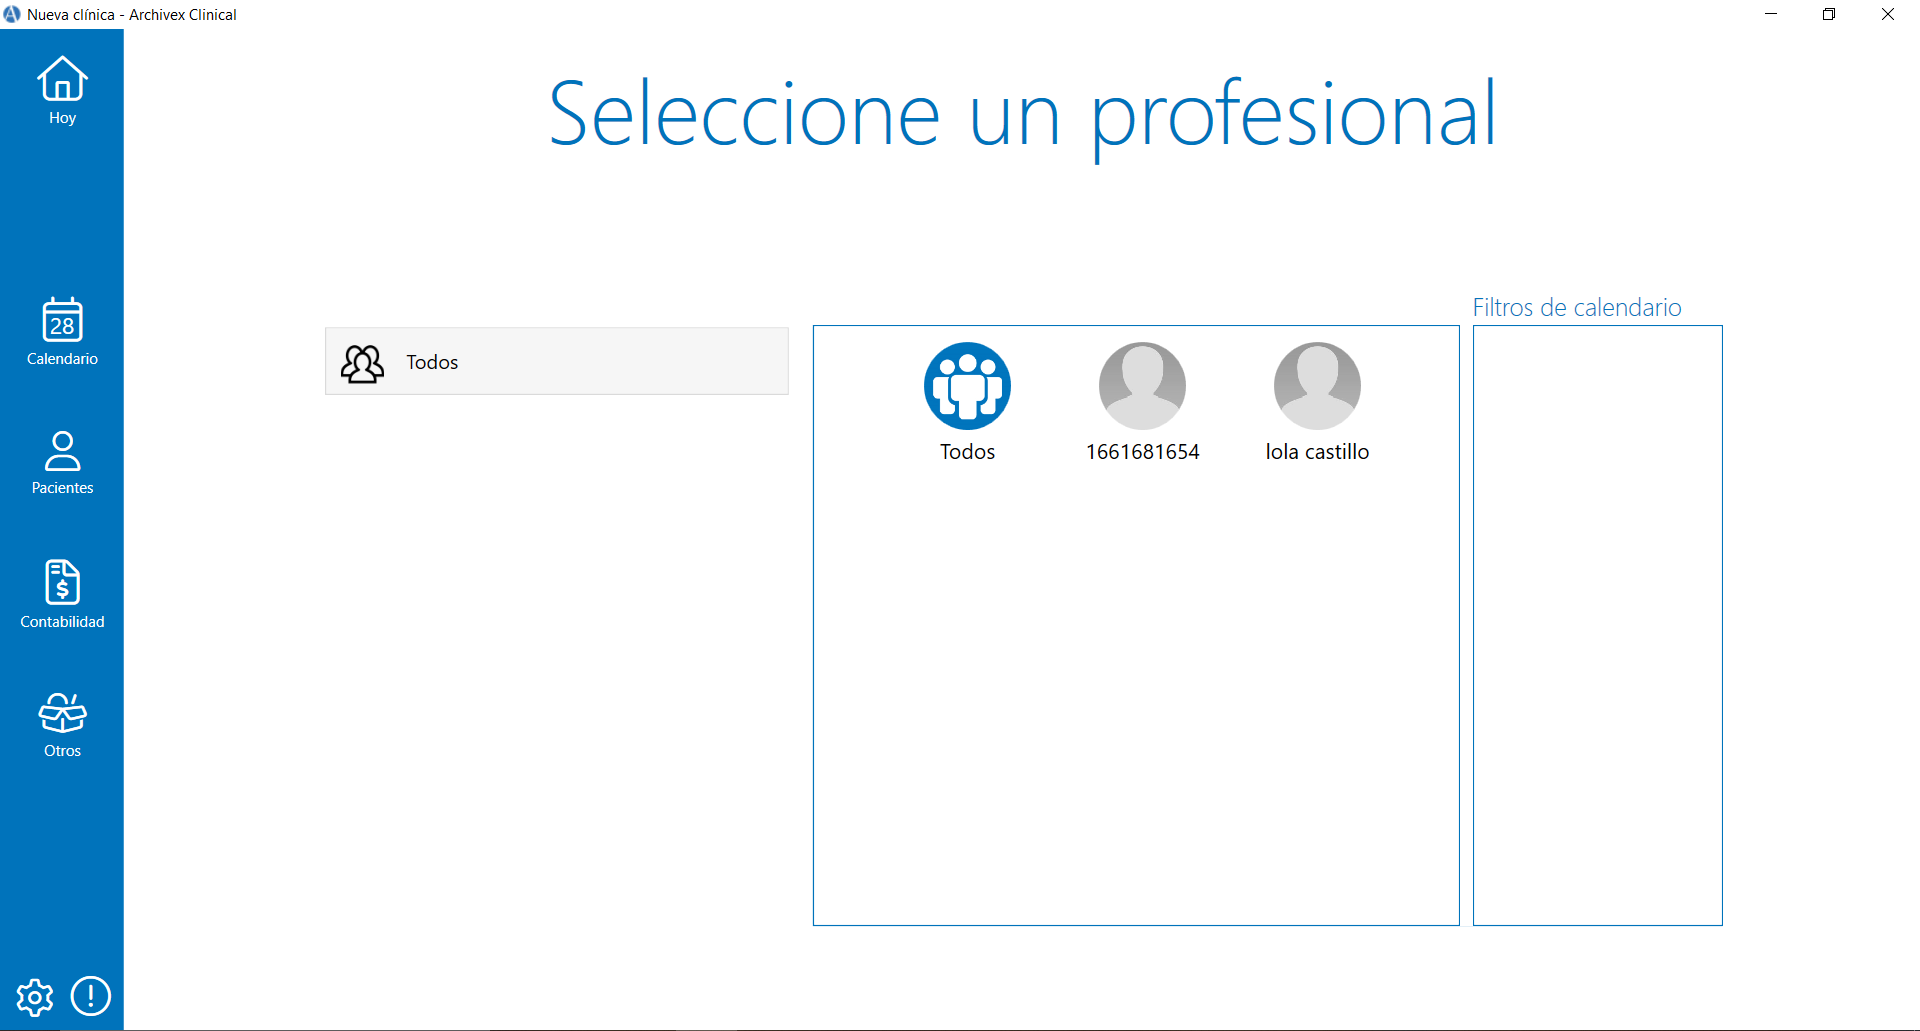
\includegraphics[scale=0.3]{doc/imagenes/archivex-calendario.png
    }}
    \caption{Vista de la sección ''Calendario''}
    \label{fig:archivex-calendario}
\end{figure}

\begin{figure}[H]
    \centering{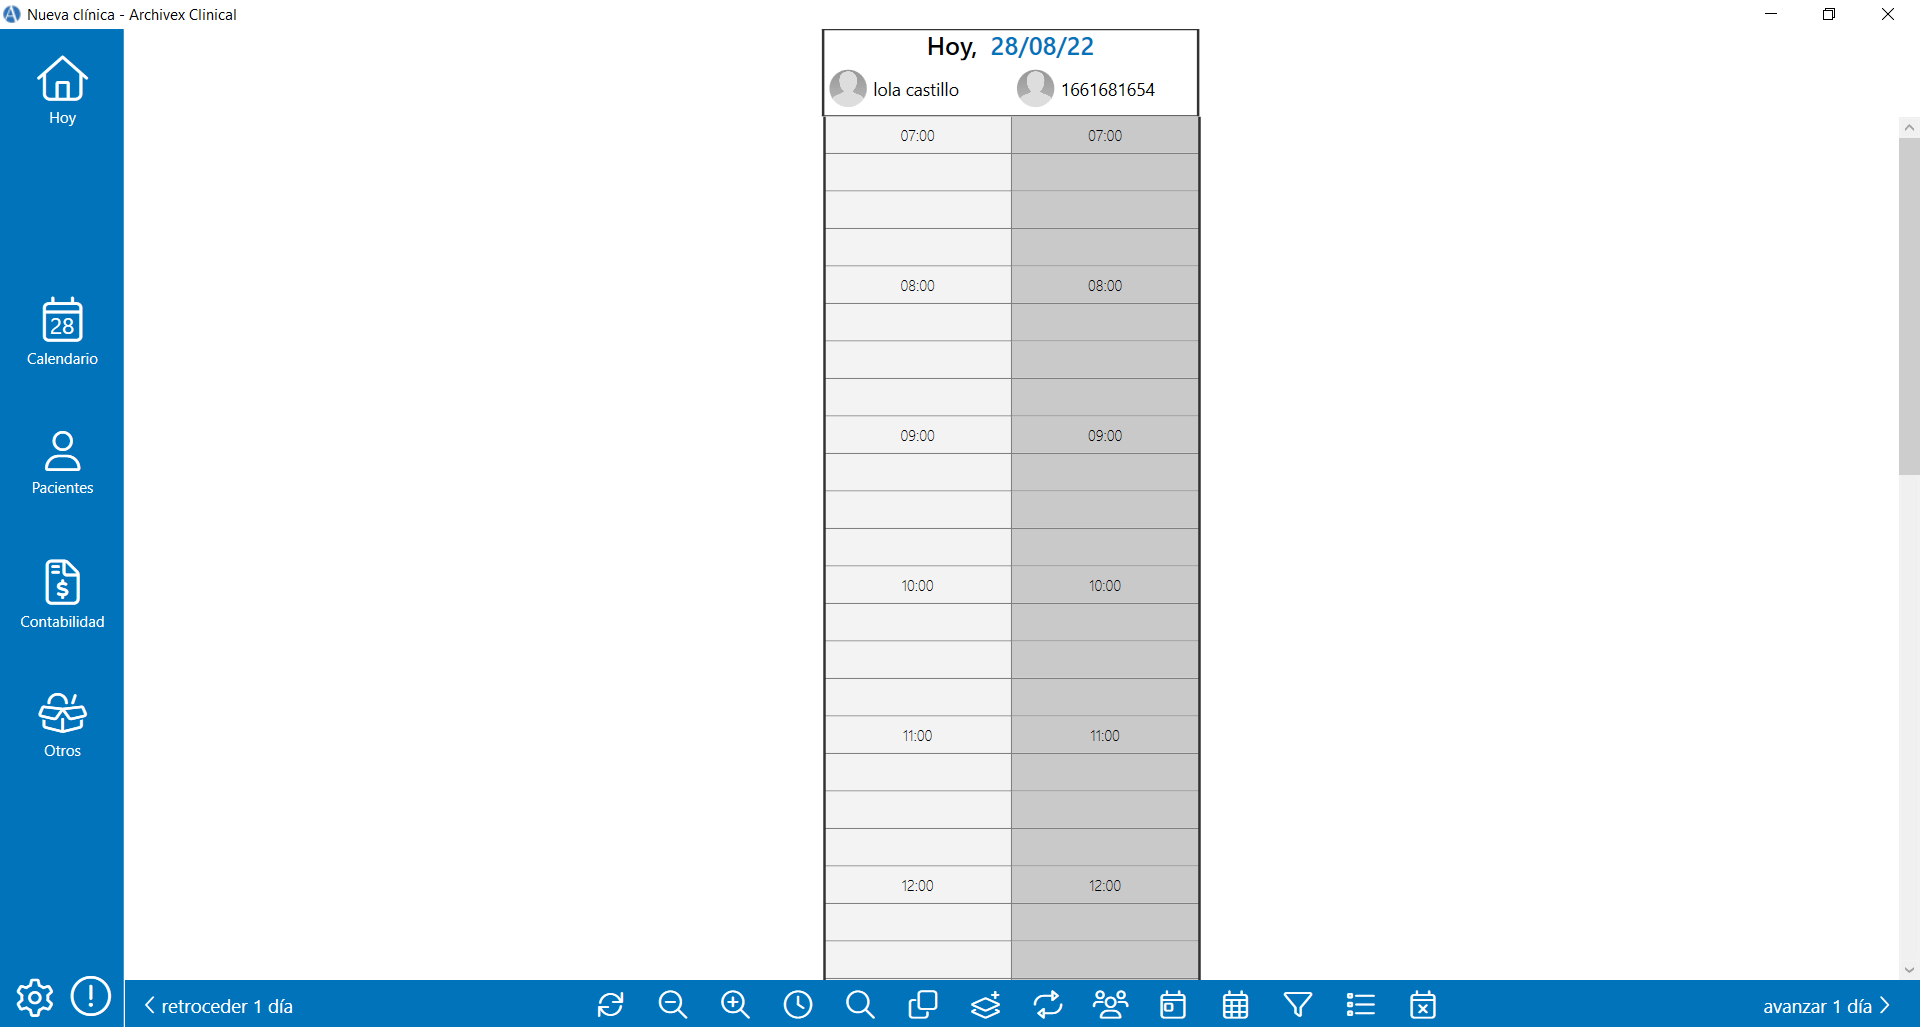
\includegraphics[scale=0.3]{doc/imagenes/archivex-agenda-todos.png
    }}
    \caption{Agenda del día actual de todos los profesionales}
    \label{fig:archivex-agenda-todos}
\end{figure}

En esta vistas en las que se muestra un calendario el usuario puede filtrar las citas por días de la semana y profesionales o avanzar o retroceder siete días (o un día si se trata de la vista de las citas de todos los profesionales). En adición a la gestión de citas, estas pueden ser notificadas a los pacientes vía WhatsApp redirigiendo al usuario al chat de WhatsApp Web asociado al número guardado en la ficha del cliente o vía SMS si se ha pagado por uno de los paquetes de pago de la Figura \ref{fig:archivex-sms} cuyo precio varía en función del número de SMS a pagar. \bigskip

\begin{figure}[H]
    \centering{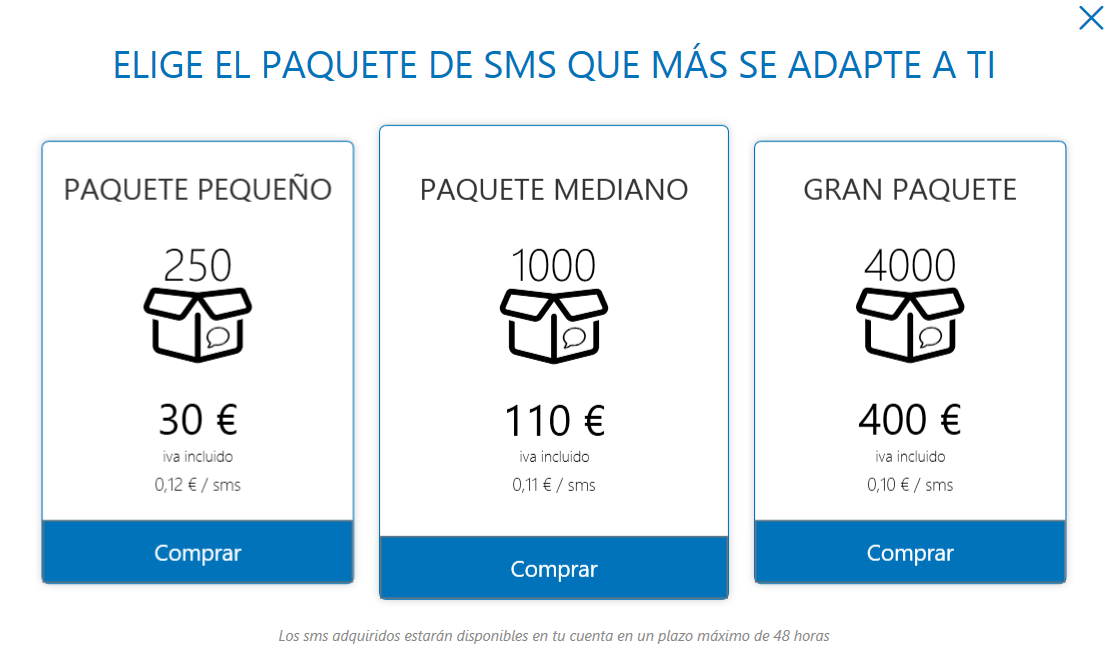
\includegraphics[scale=0.3]{doc/imagenes/archivex-sms.png
    }}
    \caption{Planes de pago de SMS}
    \label{fig:archivex-sms}
\end{figure}

Los clientes disponen con Archivex de un servicio 24 horas para gestionar sus citas. Para ello, tan sólo han de acceder a la página web de la clínica y pulsar sobre el botón de pedir cita que habrá de haber incorporado la propia clínica a su página con anterioridad. El paciente será redirigido a un inicio de sesión en el que deberá de introducir su DNI, una vez realizado esto recibirá un código por SMS o por correo electrónico que le permitirá acceder a la gestión de sus citas. En caso de que fuera su primera vez utilizando la plataforma el usuario se podrá registrar rellenando un formulario. \bigskip

A parte de la gestión de citas, Archivex también ofrece hacer una gestión del historial clínico de los pacientes, así como manejar la facturación de la clínica entre otros servicios secundarios (controlar stock, acceder a estadísticas, gestión de la información de aseguradoras, etc.). El acceso a estos servicios de acuerdo a los videos explicativos está restringido en función del rol del usuario, no obstante no se aporta más información acerca de los roles. \bigskip

En cuanto a precio, en la Figura \ref{fig:archivex-precio} se muestran los planes de pago:

\begin{figure}[H]
    \centering{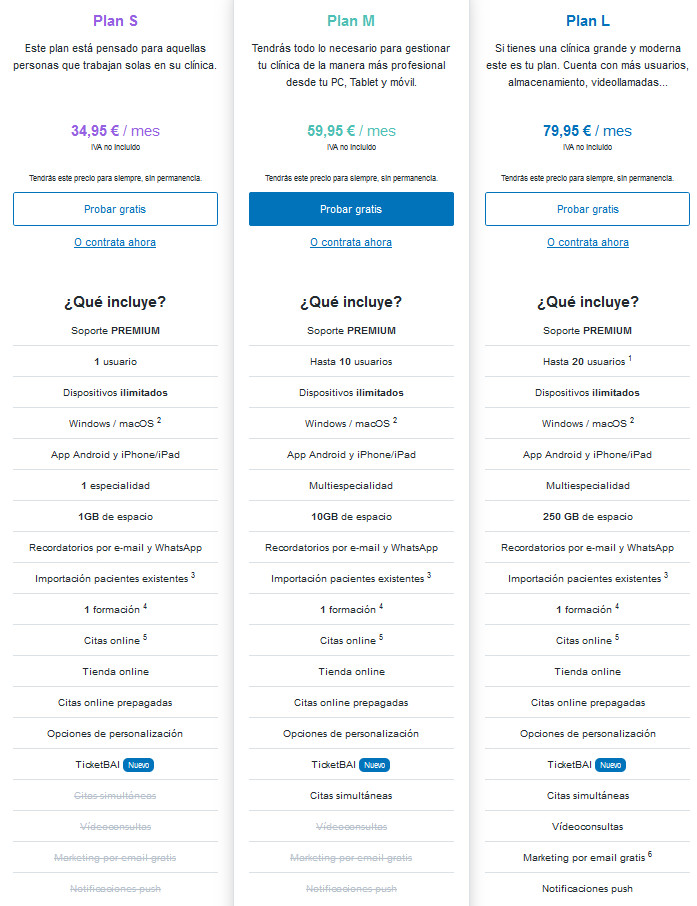
\includegraphics[scale=0.3]{doc/imagenes/archivex-precios.png
    }}
    \caption{Planes de pago de Archivex}
    \label{fig:archivex-precio}
\end{figure}

Tras conocer el servicio ofrecido por Archivex y haber probado su demo, la presentación sobre ahorro de tiempo y dinero aportada por la empresa de la herramienta no es del todo veraz. Veamos a continuación por qué:

\begin{itemize}
    \item \textbf{El tiempo}: Un usuario primerizo en el uso de la herramienta, aún visualizando los vídeos explicativos o leyendo su documentación tendría que gastar bastante de su tiempo aprendiendo a usar la herramienta. Esto se debe a que no se ofrece un tour al iniciar por primera vez sesión en la plataforma, los vídeos explicativos se centran mayormente en la gestión de citas, dejando sin cubrir otras funcionalidades como la gestión de la documentación. A esto se le suma la redundancia que aportan las vistas ''Hoy'' y ''Calendario'', una sóla vista del calendario y funciones de filtrado de citas sería suficiente. De nuevo no existe jerarquía visual, al usuario no se le indica en qué vista se encuentra y los formularios son como el de la Figura \ref{fig:archivex-crear-citas} donde se debe de hacer un recorrido visual en zigzag que aumenta la dificultad para leerlo. Además son tantos los servicios secundarios ofrecidos y la escasa documentación asociada a ellos que el usuario tendría que invertir tiempo en aprender sobre su uso. 
    \item \textbf{El dinero}: Los planes de pago se diferencian sobretodo en el espacio de almacenamiento y el número de usuarios. Aprovechar o no un plan de pago dependería en función del volumen de documentación generada por cada usuario, lo cual estaría vinculado al número de pacientes. Si se tratara de una clínica grande con un gran número de pacientes y en consecuencia con un gran número de personal el Plan L que es el que mayores ventajas aporta al usuario posiblemente no sea suficiente. En cambio en el otro extremo, Plan S, 1Gb de espacio de almacenamiento aún sólo tratándose de un usuario tampoco sería suficiente.
\end{itemize}

\begin{figure}[H]
    \centering{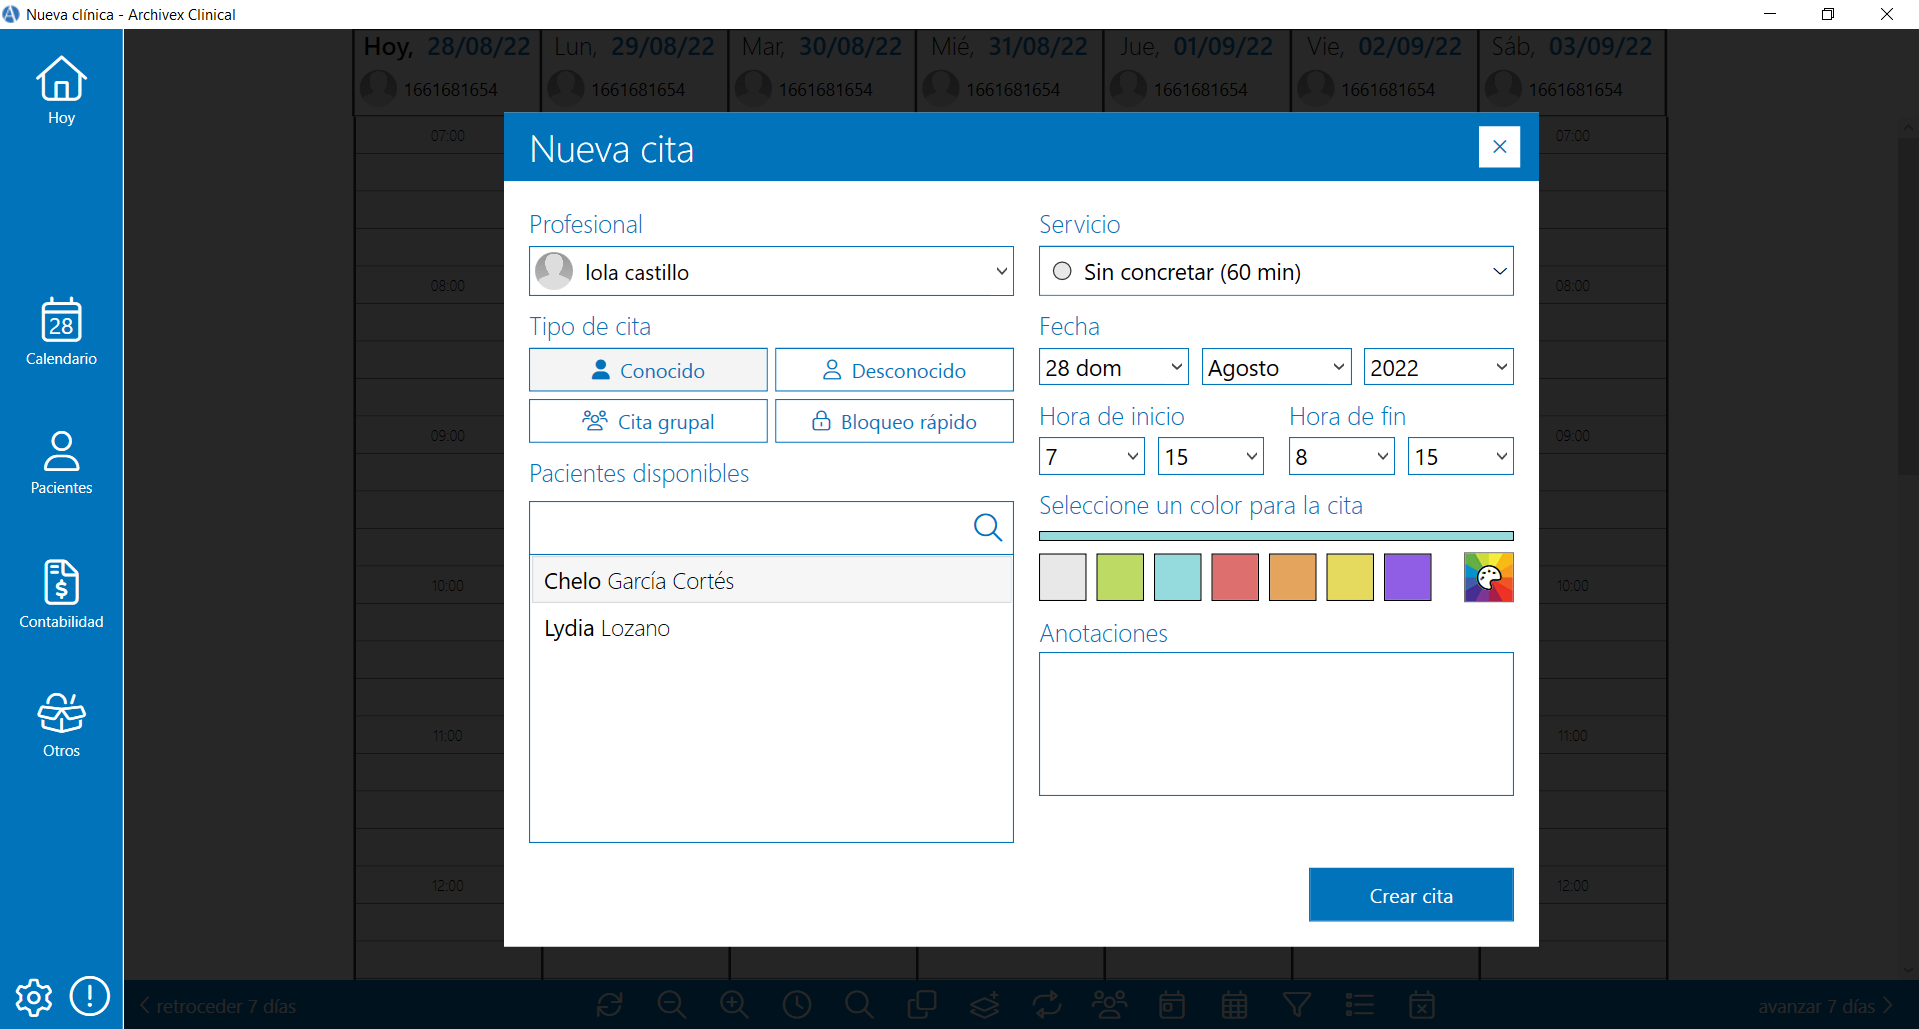
\includegraphics[scale=0.3]{doc/imagenes/archivex-crear-cita.png
    }}
    \caption{Formulario de creación de citas en Archivex}
    \label{fig:archivex-crear-citas}
\end{figure}

En conclusión después de este análisis, Archivex es un software que sería ideal por el precio y servicios ofertados para clínicas de tamaño pequeño/mediano como Carmen Verdejo contratando el Plan M o Plan L y cumpliría con su palabra de ahorro de tiempo a largo plazo cuando sus usuarios se familiarizasen más con la aplicación ya que está claro que dista de ser totalmente intuitiva. \bigskip
